\documentclass[border=3pt]{standalone}
% Preâmbulo compartilhado pelos diagramas TikZ da aula 11 (Localização por Grade e Monte Carlo)
\usepackage[T1]{fontenc}
\usepackage[utf8]{inputenc}
\usepackage{lmodern}
\usepackage{amsmath}
\usepackage{xcolor}
\usepackage{tikz}
\usetikzlibrary{arrows.meta,angles,quotes,decorations.pathmorphing,calc,
                positioning,shapes.geometric,shapes.misc,backgrounds,fit,
                math}

% Paleta (mesma dos SVGs originais)
\definecolor{dblue}{HTML}{2A5B8C}
\definecolor{dorange}{HTML}{B3541E}
\definecolor{dgreen}{HTML}{4A7C59}
\definecolor{dred}{HTML}{9C4B4B}
\definecolor{dcream}{HTML}{F4F1EA}
\definecolor{dshade}{HTML}{DDD7C9}

% Função gaussiana (não normalizada por padrão de escala visual)
\pgfmathdeclarefunction{gauss}{3}{%
  \pgfmathparse{1/(#3*sqrt(2*pi))*exp(-((#1-#2)^2)/(2*#3^2))}%
}

% Estilos comuns (prefixo d... para não colidir com chaves internas do pgf)
\tikzset{
  >={Stealth[length=2mm]},
  dguide/.style={gray!55, dashed, line width=0.4pt},
  daxis/.style={gray!60, line width=0.7pt, ->},
  dbody/.style={fill=black!3, draw=black!80, line width=1pt},
  dacc/.style={draw=dblue, line width=1pt},
  dlbl/.style={black!55, font=\small},
  dsub/.style={black!45, font=\footnotesize},
  dstate/.style={circle, draw=black!80, fill=dcream, line width=1pt,
                 minimum size=17mm, font=\large, inner sep=1pt},
  dobs/.style={circle, draw=black!80, fill=dshade, line width=1pt,
               minimum size=14mm, font=\large, inner sep=1pt},
  dbox/.style={rounded corners=2pt, draw=black!80, fill=dcream, line width=1pt,
               align=center, inner sep=6pt},
  dop/.style={circle, draw=black!80, fill=white, line width=1pt,
              minimum size=6mm, inner sep=0pt, font=\small},
  dtrans/.style={->, dblue, line width=1pt},
  dmeas/.style={->, dorange, line width=1pt},
  dcurve/.style={line width=1pt, dblue},
  dcurveb/.style={line width=1.4pt, dorange},
}

\begin{document}
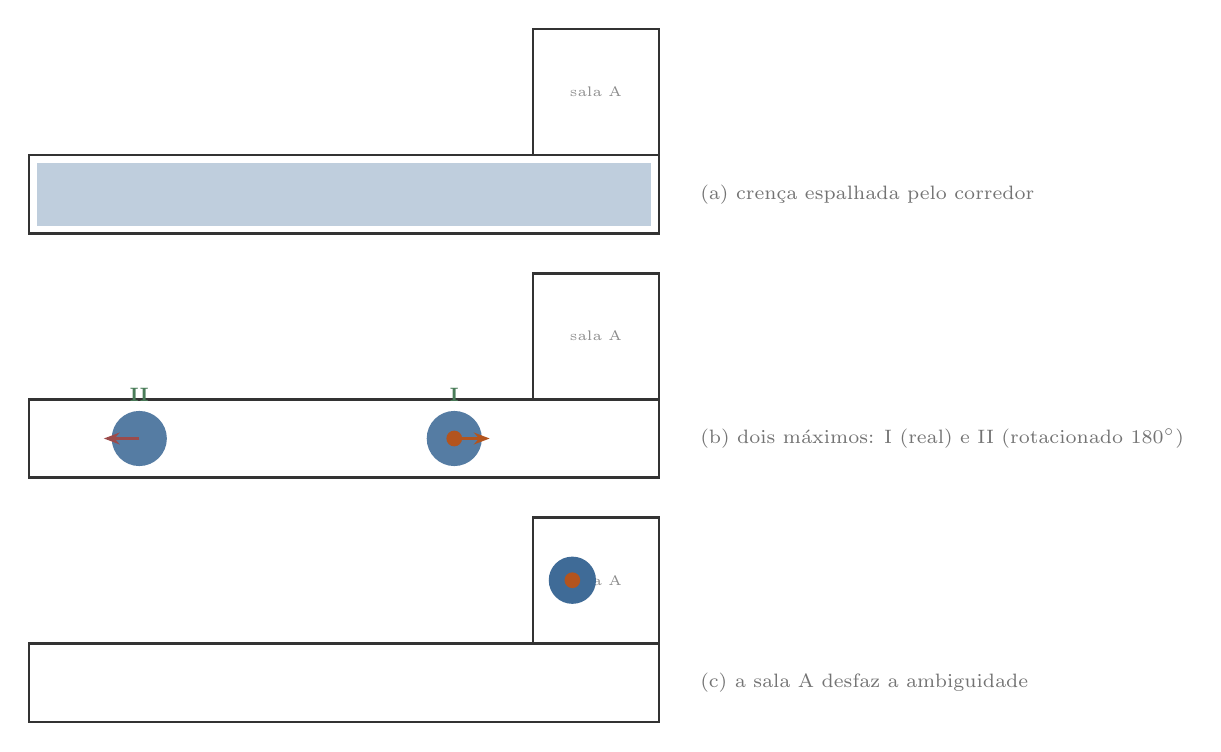
\begin{tikzpicture}[x=1cm,y=1cm]
  \newcommand{\corr}{\draw[dbody, fill=white, line width=1pt] (0,0) rectangle (8,1.0); \draw[dbody, fill=white, line width=1pt] (6.4,1.0) rectangle (8,2.6); \node[dsub, font=\tiny] at (7.2,1.8) {sala A};}
  \begin{scope}[shift={(0,6.2)}]
    \corr \fill[dblue!30] (0.1,0.1) rectangle (7.9,0.9);
    \node[dlbl, font=\scriptsize, anchor=west] at (8.4,0.5) {(a) crença espalhada pelo corredor};
  \end{scope}
  \begin{scope}[shift={(0,3.1)}]
    \corr
    \fill[dblue!80] (1.4,0.5) circle (0.35); \fill[dblue!80] (5.4,0.5) circle (0.35);
    \node[dgreen, font=\scriptsize\bfseries] at (1.4,1.05) {II};
    \node[dgreen, font=\scriptsize\bfseries] at (5.4,1.05) {I};
    \fill[dorange] (5.4,0.5) circle (0.1); \draw[->, dorange, line width=1pt] (5.4,0.5) -- (5.85,0.5);
    \draw[->, dred, line width=1pt] (1.4,0.5) -- (0.95,0.5);
    \node[dlbl, font=\scriptsize, anchor=west] at (8.4,0.5) {(b) dois máximos: I (real) e II (rotacionado 180$^\circ$)};
  \end{scope}
  \begin{scope}
    \corr
    \fill[dblue!90] (6.9,1.8) circle (0.3);
    \fill[dorange] (6.9,1.8) circle (0.1);
    \node[dlbl, font=\scriptsize, anchor=west] at (8.4,0.5) {(c) a sala A desfaz a ambiguidade};
  \end{scope}
\end{tikzpicture}
\end{document}
